% Please make sure you insert your
% data according to the instructions in PoSauthmanual.pdf
\documentclass[a4paper,11pt]{article}
\usepackage{pos}
\usepackage{amsmath,amsfonts,amssymb,eulervm,xspace}
\usepackage{amsmath,amsfonts,amssymb}
\usepackage{graphicx}
\usepackage{tikz}
\usepackage{subcaption}
\newcommand{\e}{\vec e}
\graphicspath{{../figures/}}


\title{Topology of the $O(3)$ non-linear sigma model under the gradient flow}
%% \ShortTitle{Short Title for header}

\author*[a]{Stuart Thomas}
\author[a]{Christopher Monahan}

\affiliation[a]{Department of Physics, William \& Mary,  Williamsburg, Virginia 23187, USA}

%\affiliation[b]{Department, University,\\
%Street number, City, Country}

\emailAdd{snthomas01@email.wm.edu}
\emailAdd{cjmonahan@wm.edu}

\abstract{
The $O(3)$ non-linear sigma model (NLSM) is a prototypical field theory for QCD and ferromagnetism, featuring topological qualities. Though the topological susceptibility $\chi_t$ should vanish in physical theories, lattice simulations of the NLSM find that $\chi_t$ diverges in the continuum limit. We study the effect of the gradient flow on this quantity using a Markov Chain Monte Carlo method, finding that a logarithmic divergence persists. This result supports a previous study and indicates that either the definition of topological charge is problematic or the NLSM has no well-defined continuum limit. We also introduce a $\theta$-term and analyze the topological charge as a function of $\theta$ under the gradient flow.}

\FullConference{%
 The 38th International Symposium on Lattice Field Theory, LATTICE2021
  26th-30th July, 2021
  Zoom/Gather@Massachusetts Institute of Technology
}


\begin{document}
\maketitle


\section{The Non-Linear Sigma Model}
We study the $O(3)$ non-linear sigma model (NLSM) in 1+1 dimensions, defined by the Euclidean action
\begin{equation*}
    \label{eq:nlsm euclidean action}
    S_E = \frac{\beta}{2} \int d^2x \; \left[ \left(\partial_t \e\, \right)^2+ \left( \partial_x \e\,\right)^2 \right]
\end{equation*}
where, $\e$ is 3-component real vector constrained by $|\e\,|=1$ and $\beta$ is the inverse coupling constant. In solid-state systems, this model describes Heisenberg ferromagnets \cite{callan1985} and in nuclear physics, it acts as a prototype for quantum chromodynamics (QCD), the gauge theory that describes the strong nuclear force. In general, the NLSM shares key features with non-Abelian gauge theories such as QCD, including a mass gap and asymptotic freedom \cite{polyakov1975}. Therefore, the NLSM is a useful model for exploring the effect of these properties in a simpler system.

Following~\cite{berg1981}, we define topological charge density $q(x^*)$ for each plaquette $x^*$ such that
\begin{equation}
    Q = \sum_{x^*} q(x^*)
\end{equation}
where
\begin{equation}
    q(x^*) = \frac{1}{4\pi} \bigg[A\Big(\e(x_1), \e(x_2), \e(x_3)\Big) + A\Big(\e(x_1), \e(x_3), \e(x_4)\Big) \bigg].
  \end{equation}
  The topology of the NLSM is visualized in Fig.~\ref{fig:topology}
\begin{figure}
  \centering
    \begin{subfigure}[b]{0.4\textwidth}
    \centering
    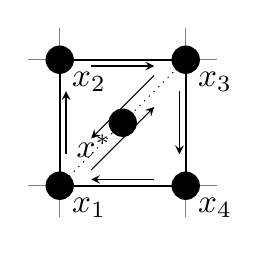
\begin{tikzpicture}[scale=0.4, every node/.style={scale=1.2}]
        \draw[step=4cm,gray,thin] (-1,-1) grid (5,5);
        \draw[dotted] (0,0) -- (4,4);
        \draw[thick](0,0) node[circle,fill,inner sep=0pt, minimum size=0.3cm]{} node[anchor=north west] {$x_1$} --
                    (0,4) node[circle,fill,inner sep=0pt, minimum size=0.3cm]{} node[anchor=north west] {$x_2$} --
                    (4,4) node[circle,fill,inner sep=0pt, minimum size=0.3cm]{} node[anchor=north west] {$x_3$} --
                    (4,0) node[circle,fill,inner sep=0pt, minimum size=0.3cm]{} node[anchor=north west] {$x_4$} -- cycle ;
                    \draw[] (2,2) node[circle,fill,inner sep=0pt, minimum size=0.3cm]{} node[anchor=north east]{$x^*$};


        \draw[-stealth] (0.2,1) -- (0.2,3);
        \draw[-stealth] (1,3.8) -- (3,3.8);
        \draw[-stealth] (3,3.5) -- (1,1.5);

        \draw[-stealth] (1,0.5) -- (3,2.5);
        \draw[-stealth] (3.8,3) -- (3.8,1);
        \draw[-stealth] (3,0.2) -- (1,0.2);
    \end{tikzpicture}
    \caption{a plaquette broken up into two triangles}
    %\caption{\label{fig:plaquette} Visualization of plaquette $x^*$. The dotted line separates the plaquette into two signed areas which are used to define the topological charge density $q(x^*)$. Arrows represent order of signed area.}
    \end{subfigure}
    \begin{subfigure}[b]{0.4\textwidth}
    \centering
    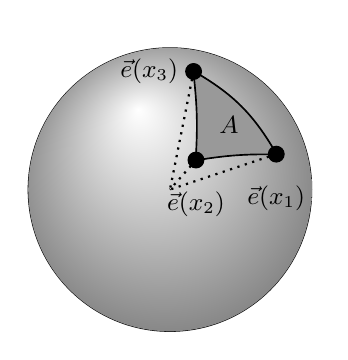
\begin{tikzpicture}[scale=0.6, every node/.style={scale=1}]
        \pgfdeclarelayer{nodelayer}
        \pgfdeclarelayer{edgelayer}
        \pgfdeclareradialshading{sphere4}{\pgfpoint{-0.2cm}{0.5cm}}%
            {rgb(0cm)=(1,1,1);
            rgb(1cm)=(0.5,0.5,0.5); rgb(1.05cm)=(1,1,1)}
            %rgb(0.7cm)=(0.1,0.1,0.1); rgb(1cm)=(0.5,0.05,0); rgb(1.05cm)=(1,1,1)}
        \pgfsetlayers{nodelayer,edgelayer}
        \tikzstyle{label}=[fill=none, draw=none, shape=circle]
        \tikzstyle{point}=[inner sep=0pt, minimum size=0.2cm,fill=black, draw, shape=circle]
        %\tikzstyle{interior line}=[{Stealth[scale=1.5]}-,dotted,thick]
        \tikzstyle{interior line}=[dotted,thick]

        \tikzstyle{triangle}=[thick]
        \tikzstyle{arrow}=[->, thick]
        \begin{pgfonlayer}{nodelayer}
            \node [style=point] (4) at (0.5, 2.5) {};
            \node [style=point] (5) at (0.55, 0.625) {};
            \node [style=point] (6) at (2.25, 0.75) {};
            \node (7) at (0, 0) {};
            \node (8) at (1.25, 1.375) {};
            \node (9) at (2.425, 2.525) {};
        \end{pgfonlayer}
        \begin{pgfonlayer}{edgelayer}
            \draw (0,0) circle (3cm);
            %\shade[inner color=white,outer color=lightgray] (0,0) circle (3cm);
            \shade[shading=sphere4] (0,0) circle (3cm);
            \draw [bend left=15,style=triangle] (4.center) to (6.center);
            \draw [bend left=355,style=triangle] (6.center) to (5.center);
            \draw [bend right=5,style=triangle] (5.center) to (4.center);
            \draw [style=interior line] (4.center) to (7.center);
            \draw [style=interior line] (5.center) to (7.center);
            \draw [style=interior line] (6.center) to (7.center);
            \draw [fill=gray!80] (4.center) to [bend left=15] (6.center) to [bend left=355] (5.center) to [bend right=5] cycle;

            %\draw [style=arrow] (8.center) to (9.center);

            \node [style=label, anchor=north] at (2.25, 0.75) {\small $\e(x_1)$};
            \node [style=label, anchor=north] at (0.55, 0.625) {\small $\e(x_2)$};
            \node [style=label, anchor=east] at (0.5, 2.5) {\small $\e(x_3)$};
            \node [style=point] at (4){};
            \node [style=point] at (5){};
            \node [style=point] at (6){};

            \node [style=label] at (8) {\small $A$};
        \end{pgfonlayer}
    \end{tikzpicture}
    \caption{signed area of triangle in target space}
    \end{subfigure}
    \caption{\label{fig:topology}}
\end{figure}

\begin{equation*}
    S[\e\,] \rightarrow S[\e\,] - i \theta Q[\e\,].
\end{equation*}
A nonzero $\theta$ implies nonzero $\langle Q \rangle$. Furthermore,
\begin{equation}
    \chi_t \propto \left. \frac{d\,\mathrm{Im}\langle Q \rangle}{d\theta}\right|_{\theta=0}
\end{equation}

\section{Computational Methods}
Our study of the gradient flow in the NLSM is based on a computational system that simulates quantum fields numerically. We begin by implementing a numerical Monte Carlo method to simulate the lattice in two dimensions and verify our program with the well-studied $\phi^4$ scalar field theory. We then generalize our model to a vector field to simulate the NLSM and implement a numerical solution to the gradient flow. We use the data produced by this program to study the topological charge and susceptibility under the gradient flow.

We first implement the $\phi^4$ model in Python. Afterwards, we transition to the NLSM, using C++ for increased efficiency . To compile the C++ simulation, we use the \texttt{gcc} compiler with the highest level of optimization.

\section{Results}
\begin{figure}[h!]
    \begin{center}
        \begin{subfigure}[b]{0.45\textwidth}
            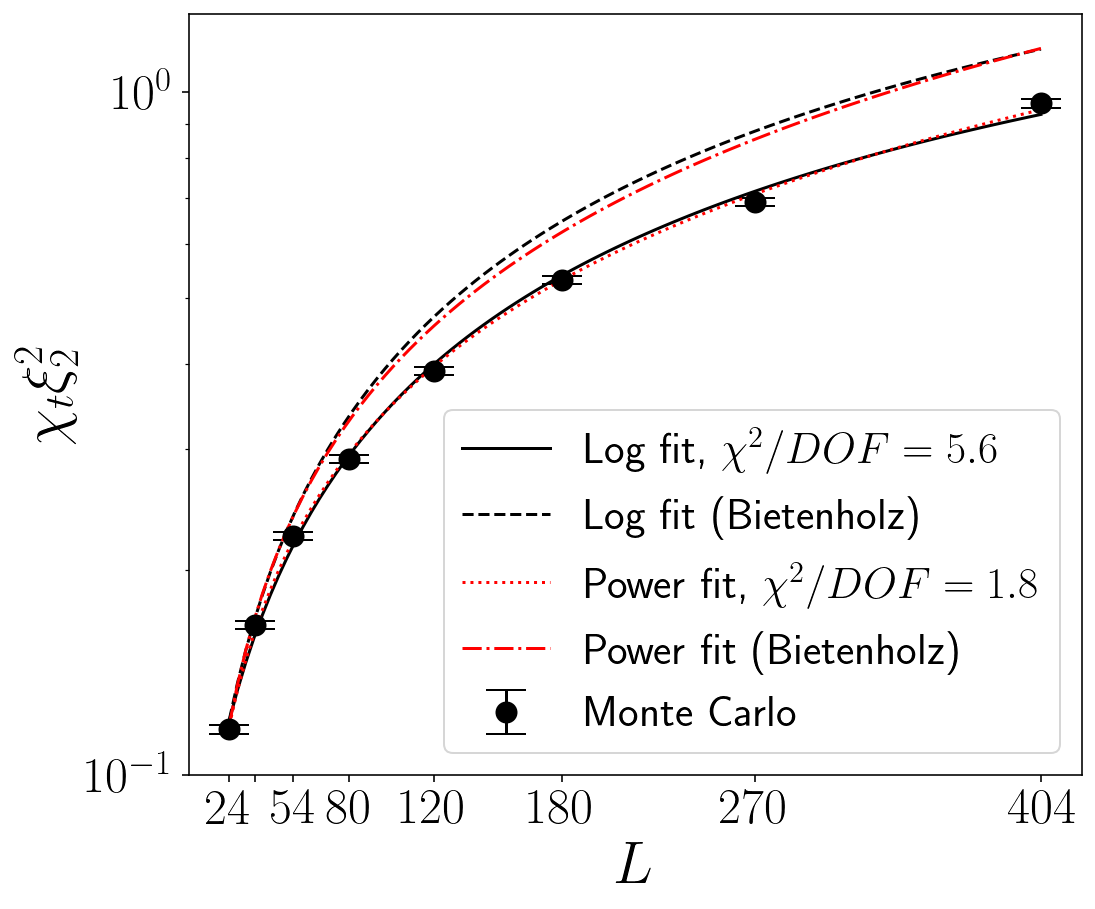
\includegraphics[height=0.7\textwidth]{divergence.png}
            \caption{$\tau = 0$}
        \end{subfigure}%
        \begin{subfigure}[b]{0.45\textwidth}
            \centering
            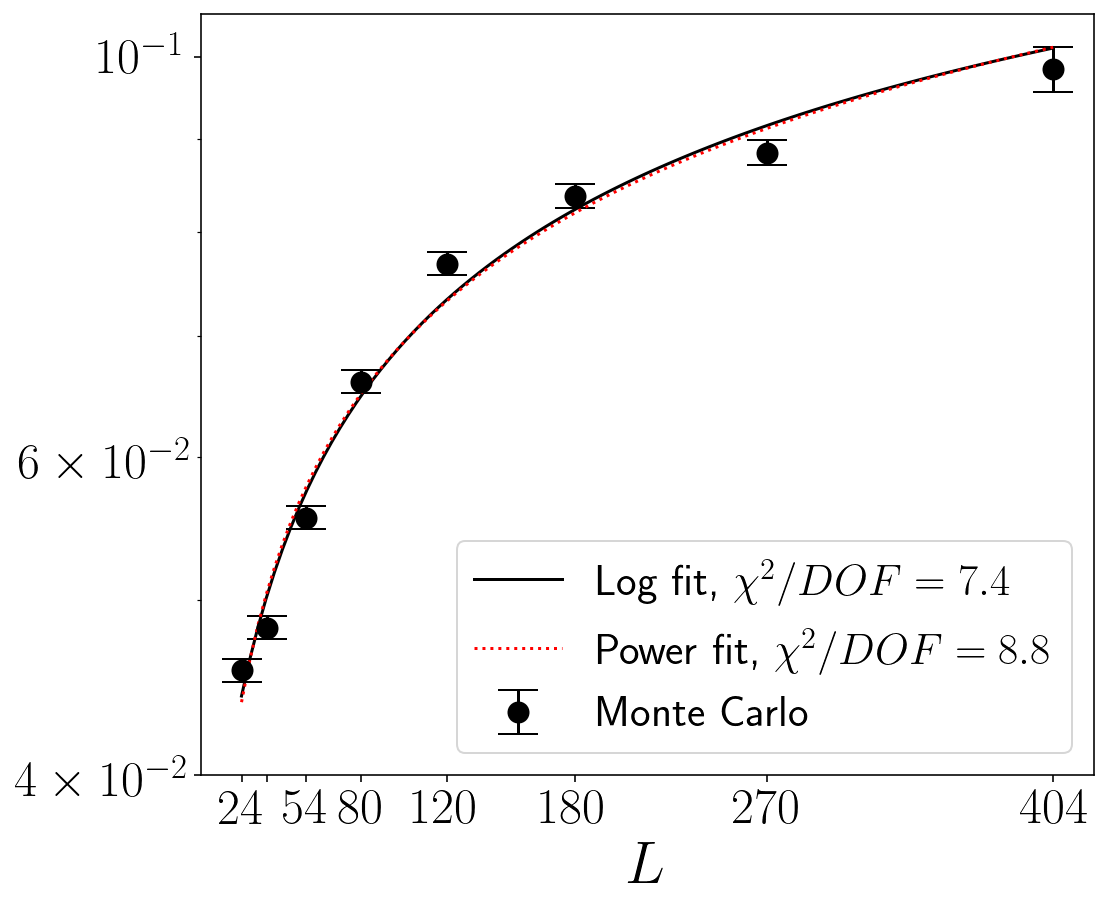
\includegraphics[height=0.7\textwidth]{divergence_flowed.png}
            \caption{$\tau = 5t_0$}
        \end{subfigure}
    \end{center}
        \caption{\label{fig:divergence} $\chi_t\xi_2^2$ as a function of $L$. $\xi_2$ is the second moment of the correlation function and $t_0$ is a scale-independent unit of flow time. We fit the data with both a logarithmic and power fit. Simulation run with 10,000 measurements every 50 sweeps, 1,000 sweep thermalization. In the $\tau=0$ case, we have compared our result with the curve fits found in \cite{bietenholz2018}.}
        %\caption{Divergent properties with
        %comparison to~\footfullcite{bietenholz2018}, 10,000 measurements}
\end{figure}

\begin{figure}[h]
    \centering
    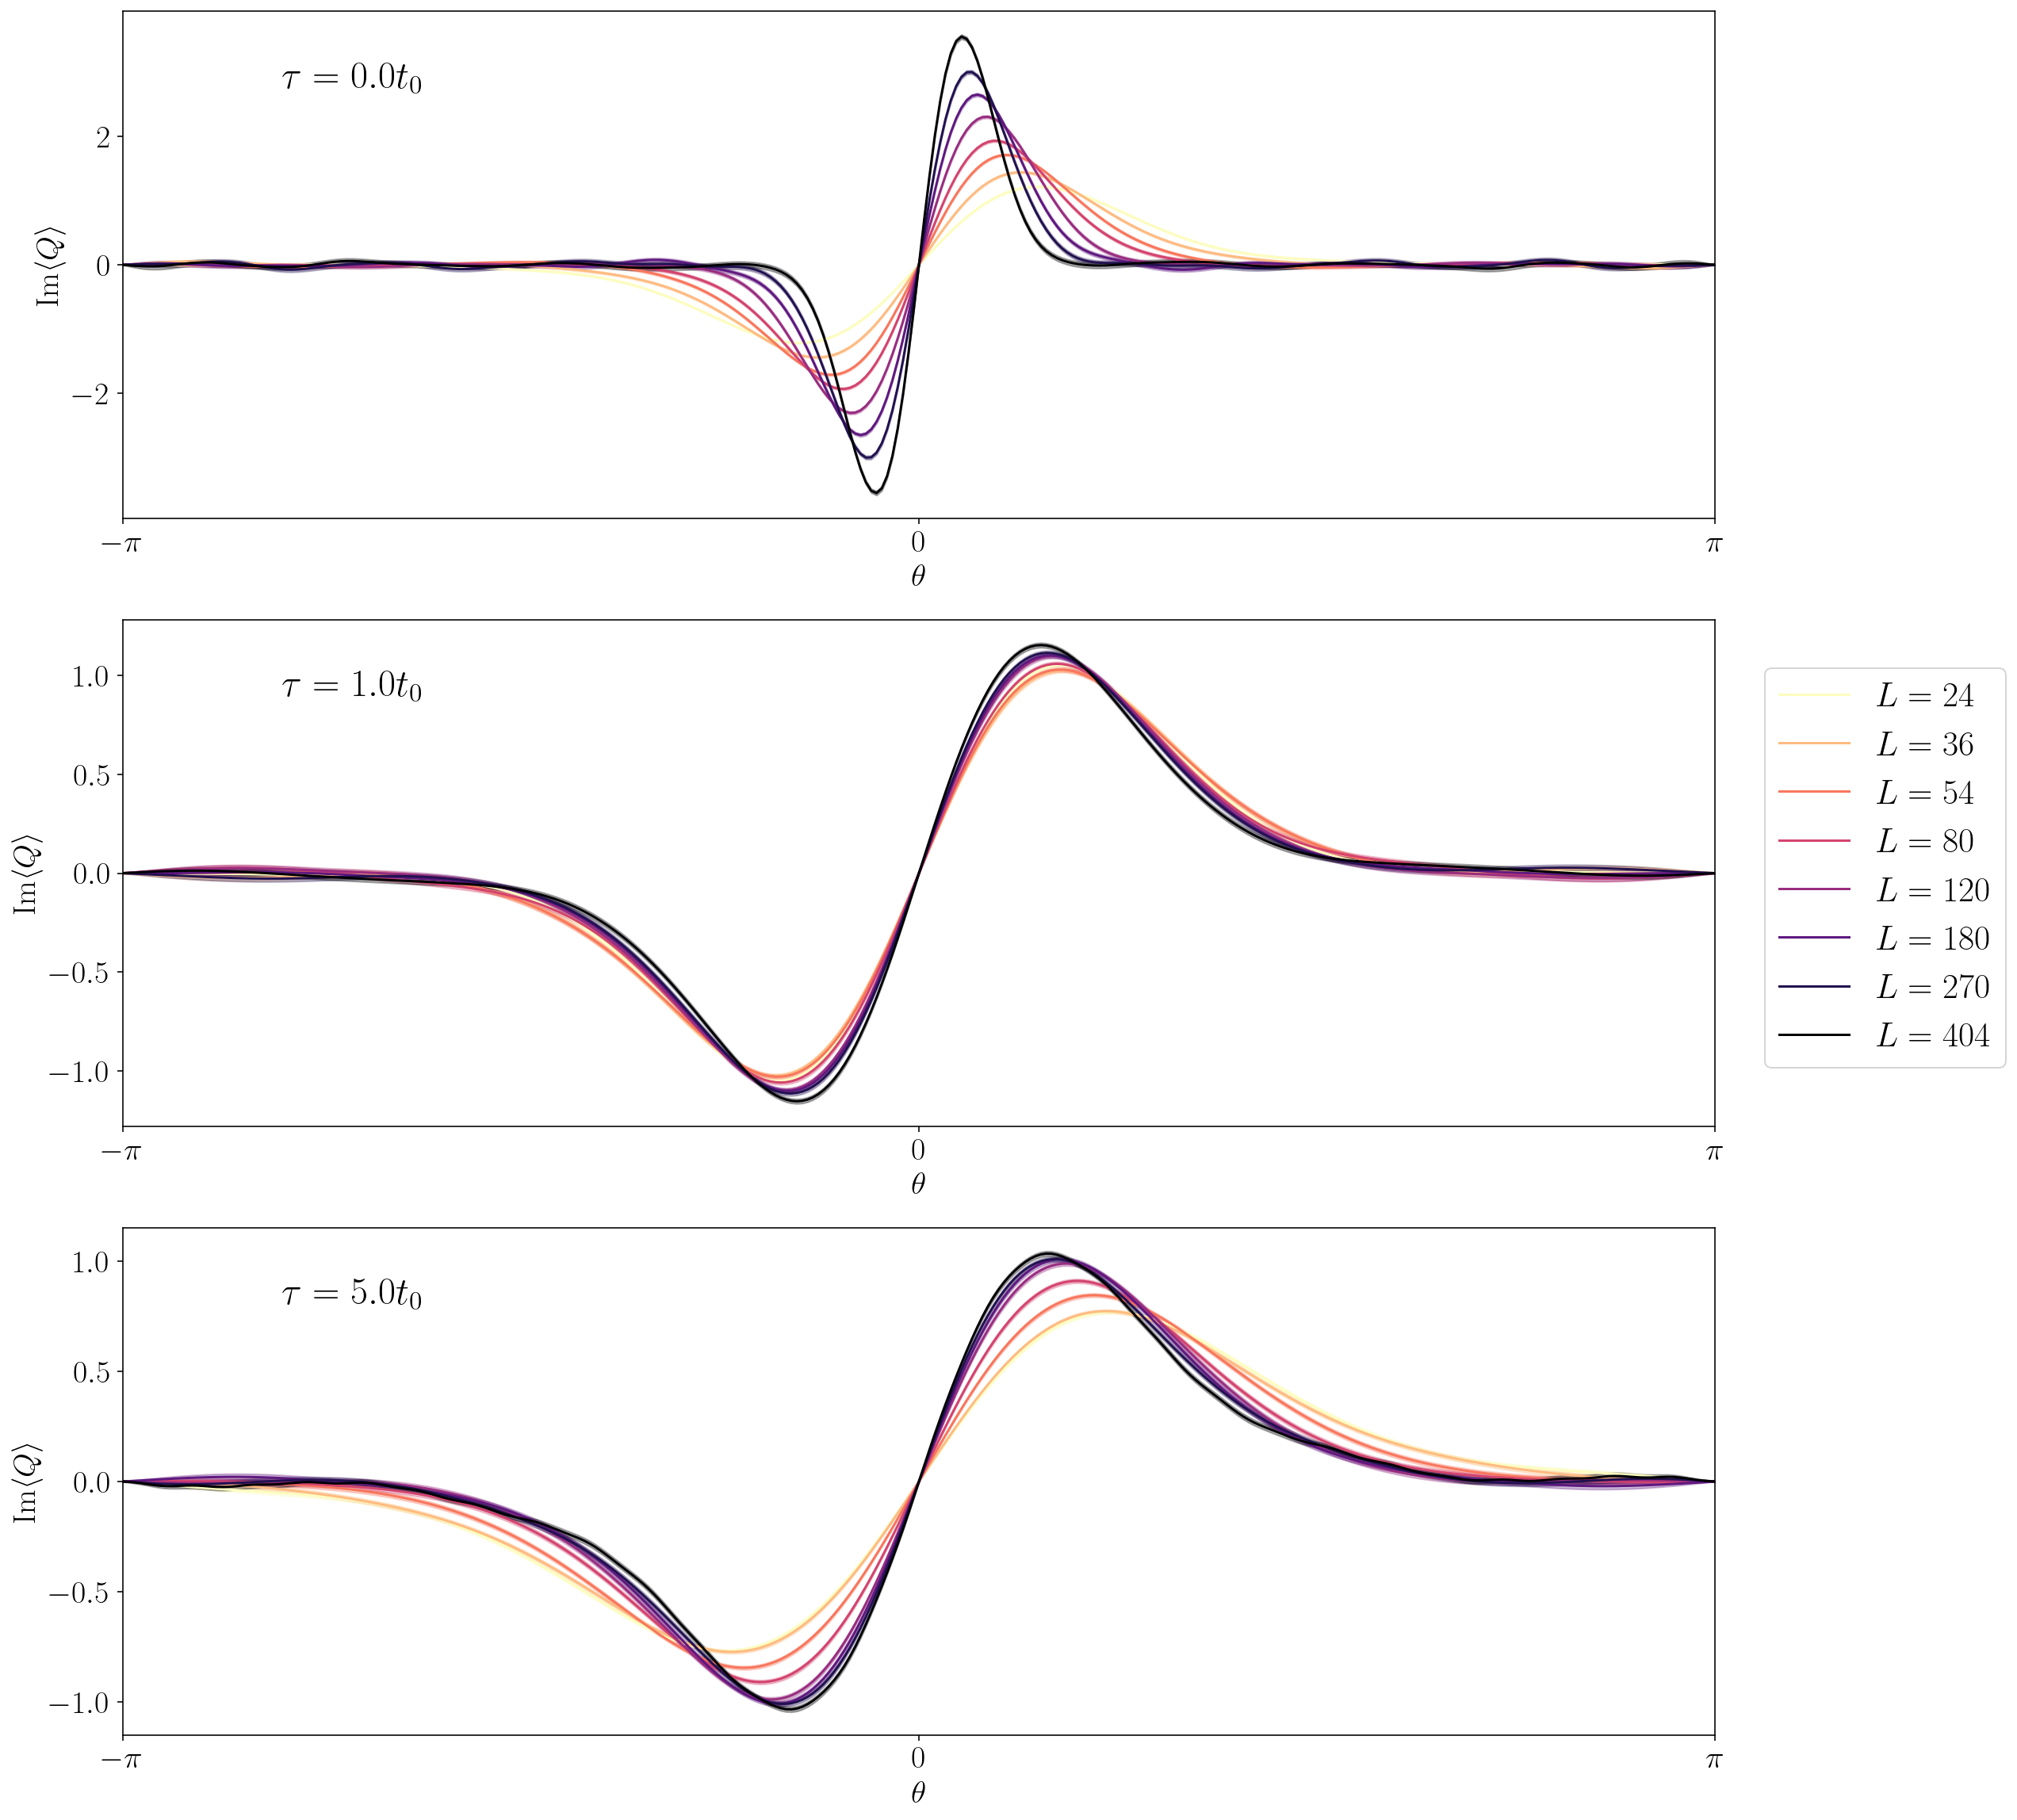
\includegraphics[width=0.5\textwidth]{theta.png}
    \caption{\label{fig:theta} Nontrivial $\mathrm{Im}\langle Q \rangle$ as a function of $\theta$. Simulation run with 10,000 measurements, every 50 sweeps, 1,000 sweep thermalization. Note the different scaling of the $y$-axis.}
  \end{figure}


\bibliographystyle{JHEP}
\bibliography{library}
\end{document}
